\documentclass[a4paper,bibliography=totoc]{scrartcl}
\usepackage[a4paper,margin=2.5cm]{geometry}
\usepackage[utf8]{inputenc}
\usepackage[english]{babel}
\usepackage[super]{natbib}
\usepackage[symbol]{footmisc}
\usepackage[htt]{hyphenat}
\usepackage{paralist}
\usepackage{abstract}
\usepackage{longtable}
\usepackage{array}
\usepackage{graphicx}
\usepackage{subfig}
\usepackage{lmodern}
\usepackage{hyperref}
\usepackage{tikz}
\usepackage{makecell}
\usepackage{xspace}
\usepackage{multirow}
\usepackage{svg}
\usepackage[section]{placeins}
\usetikzlibrary{shapes.geometric, arrows, positioning}

\usepackage{listings}
\usepackage{textcomp}
\usepackage{color}

%
% ECMAScript 2015 (ES6) definition by Gary Hammock
%

\lstdefinelanguage[ECMAScript2015]{JavaScript}[]{JavaScript}{
  morekeywords=[1]{await, async, case, catch, class, const, default, do,
    enum, export, extends, finally, from, implements, import, instanceof,
    let, static, super, switch, throw, try},
  morestring=[b]` % Interpolation strings.
}


%
% JavaScript version 1.1 by Gary Hammock
%
% Reference:
%   B. Eich and C. Rand Mckinney, "JavaScript Language Specification
%     (Preliminary Draft)", JavaScript 1.1.  1996-11-18.  [Online]
%     http://hepunx.rl.ac.uk/~adye/jsspec11/titlepg2.htm
%

\lstdefinelanguage{JavaScript}{
  morekeywords=[1]{break, continue, delete, else, for, function, if, in,
    new, return, this, typeof, var, void, while, with},
  % Literals, primitive types, and reference types.
  morekeywords=[2]{false, null, true, boolean, number, undefined,
    Array, Boolean, Date, Math, Number, String, Object},
  % Built-ins.
  morekeywords=[3]{eval, parseInt, parseFloat, escape, unescape},
  sensitive,
  morecomment=[s]{/*}{*/},
  morecomment=[l]//,
  morecomment=[s]{/**}{*/}, % JavaDoc style comments
  morestring=[b]',
  morestring=[b]"
}[keywords, comments, strings]


\lstalias[]{ES6}[ECMAScript2015]{JavaScript}

% Requires package: color.
\definecolor{mediumgray}{rgb}{0.3, 0.4, 0.4}
\definecolor{mediumblue}{rgb}{0.0, 0.0, 0.8}
\definecolor{forestgreen}{rgb}{0.13, 0.55, 0.13}
\definecolor{darkviolet}{rgb}{0.58, 0.0, 0.83}
\definecolor{royalblue}{rgb}{0.25, 0.41, 0.88}
\definecolor{crimson}{rgb}{0.86, 0.8, 0.24}

\lstdefinestyle{JSES6Base}{
  backgroundcolor=\color{white},
  basicstyle=\ttfamily,
  breakatwhitespace=false,
  breaklines=true`',
  columns=fullflexible,
  commentstyle=\color{mediumgray}\upshape,
  emph={},
  emphstyle=\color{crimson},
  extendedchars=true,  % requires inputenc
  fontadjust=true,
  frame=single,
  identifierstyle=\color{black},
  keepspaces=true,
  keywordstyle=\color{mediumblue},
  keywordstyle={[2]\color{darkviolet}},
  keywordstyle={[3]\color{royalblue}},
  numbers=left,
  numbersep=5pt,
  numberstyle=\tiny\color{black},
  rulecolor=\color{black},
  showlines=true,
  showspaces=false,
  showstringspaces=false,
  showtabs=false,
  stringstyle=\color{forestgreen},
  tabsize=2,
  upquote=true  % requires textcomp
}

\lstdefinestyle{JavaScript}{
  language=JavaScript,
  style=JSES6Base
}
\lstdefinestyle{ES6}{
  language=ES6,
  style=JSES6Base
}

\lstdefinestyle{json}{
  backgroundcolor=\color{white},
  basicstyle=\ttfamily,
  breakatwhitespace=false,
  breaklines=true`',
  columns=fullflexible,
  comment=[l]{:},
  commentstyle=\color{mediumgray}\upshape,
  emph={},
  emphstyle=\color{crimson},
  extendedchars=true,  % requires inputenc
  fontadjust=true,
  frame=single,
  identifierstyle=\color{black},
  keepspaces=true,
  numbers=left,
  numbersep=5pt,
  numberstyle=\tiny\color{black},
  rulecolor=\color{black},
  showlines=true,
  showspaces=false,
  showstringspaces=false,
  showtabs=false,
  string=[s]{"}{"},
  stringstyle=\color{royalblue},
  tabsize=2,
  upquote=true  % requires textcomp
}

\newcommand{\Azure}{Microsoft Azure\xspace}
\newcommand{\GCP}{Google Cloud Platform\xspace}
\newcommand{\AWS}{Amazon Web Services\xspace}

\begin{document}

\begin{titlepage}\centering\Large
    
\includegraphics[width=5cm]{uibk_logo.pdf}
    \vfill
    DPS Research Seminar\\Winter Term 2022/23
    \vfill
    {\titlefont\huge File Transfer Performance\\of\\Cloud Providers}
    \vfill
    Manuel Meitinger, BSc
    \vfill
\end{titlepage}

\begin{abstract}
Scheduling in the cloud focuses primarily on costs and compute resources. It is often assumed that within the same region, file transfers perform equally well between intra-provider endpoints. Inter-region transfers are usually modelled in a content-agnostic way and assuming symmetric bandwidths. This seminar paper will analyze multiple cloud providers, regions and services to uncover differences in file transfer performance, that can aid future scheduling decisions.
\end{abstract}

\vfill

\tableofcontents

\vfill

\newpage

\section{Introduction}
The possible benefits of multi-cloud approaches have long been realised,\cite{multi_cloud_expectations} and over the last decade, public cloud providers like \AWS, \Azure and \GCP continuously improved various service models.\cite{public_cloud_comparison} A more recent and fast growing model, serverless computing, alleviates the burden of managing VMs and software stacks, and instead allows to focus on scheduling.\cite{multi_cloud_serverless} However, research regarding scheduling predominantly gravitates towards compute-intense tasks and often neglects storage transfer performance.\cite{serverless_computing_and_scheduling}\\
In single-cloud environments, scheduling also tends to either focus on intra-region transfers between VM hosts and storage,\cite{network_aware_vm_migration,content_based_scheduling_vm} or assumes symmetric inter-region bandwidth.\cite{twin_sibling_faas}\\
The contribution of this work is to provide
\begin{inparaenum}[(i)]
    \item insights in multi-cloud, multi-region transfer performance and capabilities that can aid scheduling,
    \item a test environment that allows to reproduce the results as well as rapid development and execution of additional tests, and
    \item 162k publicly available data points measuring the performance across 77 regions and three providers.
\end{inparaenum}

\subsection{Related Work}
While existing measurement data is hard to find, Imran et al. addressed scheduling with explicit focus on transfer performance in \textit{OneDataShare}.\cite{data_transfer_scheduling} Their testbed and approach supports multi-cloud in theory, yet they only conducted tests on \AWS. Also, unlike more cloud-oriented services like Function as a Service (FaaS), where scheduling decides which function in which region to execute,\cite{faas_introduction} the scheduling services considered in \textit{OneDataShare} operate on transfer parameters, like compression, buffer size or transmission protocol. In our work we look at compression as well, but otherwise assume HTTPS for all transfers.\\
Serhiienko and Spillner looked at the performance of multi-cloud management platforms,\cite{recomputable_comarison_multi_cloud_platforms} where they also measured different download and upload times of files ranging from bytes to megabytes in size, using a recomputable method. In contrast to our work, they performed no inter-cloud or inter-region transfers, as they compared multi-cloud-targeting libraries within a single cloud provider and region.

\section{File Transfer and Storage Capabilities}
Before we evaluate the performance of each cloud provider, we need to understand what kind of transfers we are actually able to measure, where endpoints reside, and what storage capabilities are available. Also, a file transfer endpoint isn't just a bucket or container (or more precise: the storage service), but other file-based services as well. Performing optical character recognition (OCR) in the cloud, for example, requires a file to be transferred to that service.\cite{aws_rekognition,azure_ocr,gcp_annotate}\\
Nonetheless, let's start by covering the storage services first.

\subsection{Folders and Files}\label{sec:files_and_folders}
Each of the three cloud providers have their own storage solution for files. Files are also called objects on \AWS\cite{aws_s3_objects} and \GCP\cite{gcp_storage_objects} or blobs on \Azure\cite{azure_blob_storage}. These files are stored within buckets (\AWS, \GCP) or containers (\Azure), at a specific geographical region (\AWS, \GCP) or location (\Azure). All three storage services support role-based and policy-based access control on bucket (or container) level.\cite{aws_s3_security,azure_storage_security,gcp_storage_security}. It should be noted that objects in buckets (or blobs in containers) follow a flat structure, but all providers support a logical folder hierarchy.\cite{aws_s3_folders,gcp_storage_buckets} Different storage classes (also called access tiers) are available, influencing availability by redundancy and retrieval time.\cite{aws_s3_classes,azure_storage_tiers,gcp_storage_classes}\\
For our tests we opted to use a per-bucket (per-container) public access policy and a hot (or standard) storage class. Using a public access policy allows all files to be downloaded using a publicly accessible URL, which has the advantage of being able to directly measure transfer times, without having any authorization or storage API overhead. Using hot storage keeps the retrieval latency at a minimum, thus also favoring pure transfer times.\\
In addition, no multi-region redundancy has been used, and - where available - also no multi-zone redundancy, in order to precisely limit the origin of the transfer.

\subsection{Endpoints and Regions}\label{sec:endpoints}
Up to now, we've only talked about publicly accessible URLs for files, but not how they work on the different providers, i.e. what the storage service's endpoint looks like.
\begin{description}
    \item[\AWS:] \texttt{https://<bucket>.<region>.amazonaws.com/<object>}\cite{aws_s3_access}\\
    The region is part of the endpoint's host name, which also resolves to an IP address in that particular region. 
    \item[\Azure:] \texttt{https://<storageaccount>.blob.core.windows.net/<container>/<blob>}\cite{azure_storage_access}\\
    The last subdomain is the name of the container's \textit{storage account}, which is a collection of containers (and other storage solutions), and is also bound to a specific region.\cite{azure_storage_accounts} When a client resolves the storage account endpoint's host name, it gets a \texttt{CNAME} entry to another host that resides in that region and has an IP address in that particular region as well.
    \item[\GCP:] \texttt{https://storage.googleapis.com/<bucket>/<object>}\cite{gcp_storage_acces}\\
    Unlike \AWS and \Azure, \GCP uses \textit{anycast} IP addresses.\cite{cloudflare_anycast} So from outside of Google's network, it is not possible to deduce the region of the bucket by tools like IP geolocation, as the returned IP address will be routed by BGP to the nearest data center, and then internally by Google.\\
    However, when \texttt{storage.googleapis.com} is resolved within \GCP, say from a Cloud Function, a \texttt{CNAME} to an internal storage handling server is returned. So for example in region \textit{europe-west3} (which is located in Frankfurt) the host name \texttt{fra24s05-in-x10.1e100.net} is returned, which has a region-bound IP address instead of an anycast one. As these host names can be accessed from anywhere within the \GCP, it is possible to 'enforce' a specific endpoint region. Also, IP geolocation is again possible.
\end{description}
Figure \ref{fig:regions} was composed using geolocation tools and publicly available information.\cite{aws_regions,azure_regions,gcp_regions} It depicts all considered regions and locations.
\begin{figure}[!ht]
    \centering
    \subfloat[\centering \AWS]{{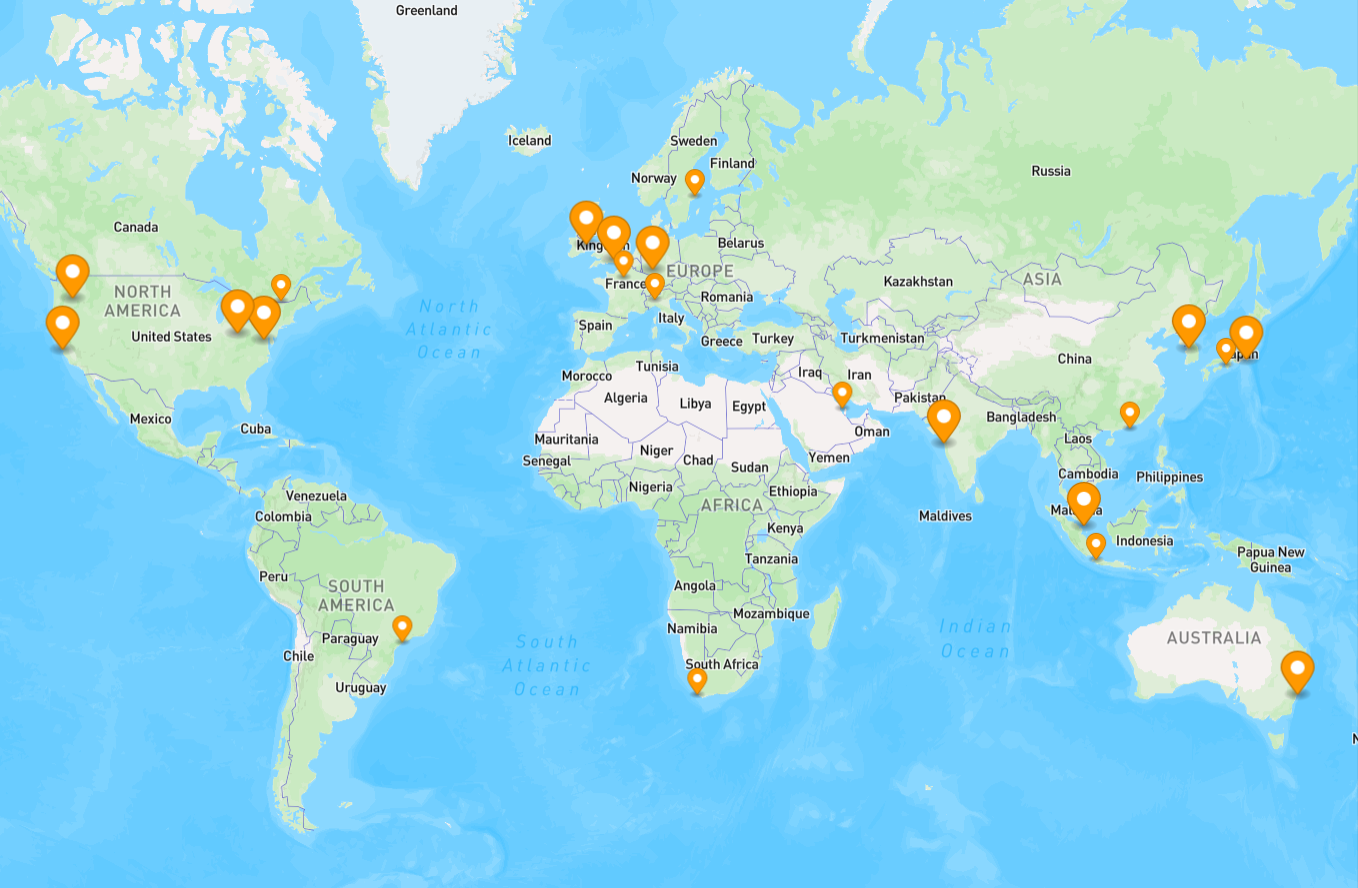
\includegraphics[width=7.5cm]{charts/datacenters_aws.png}}}%
    \qquad
    \subfloat[\centering \Azure]{{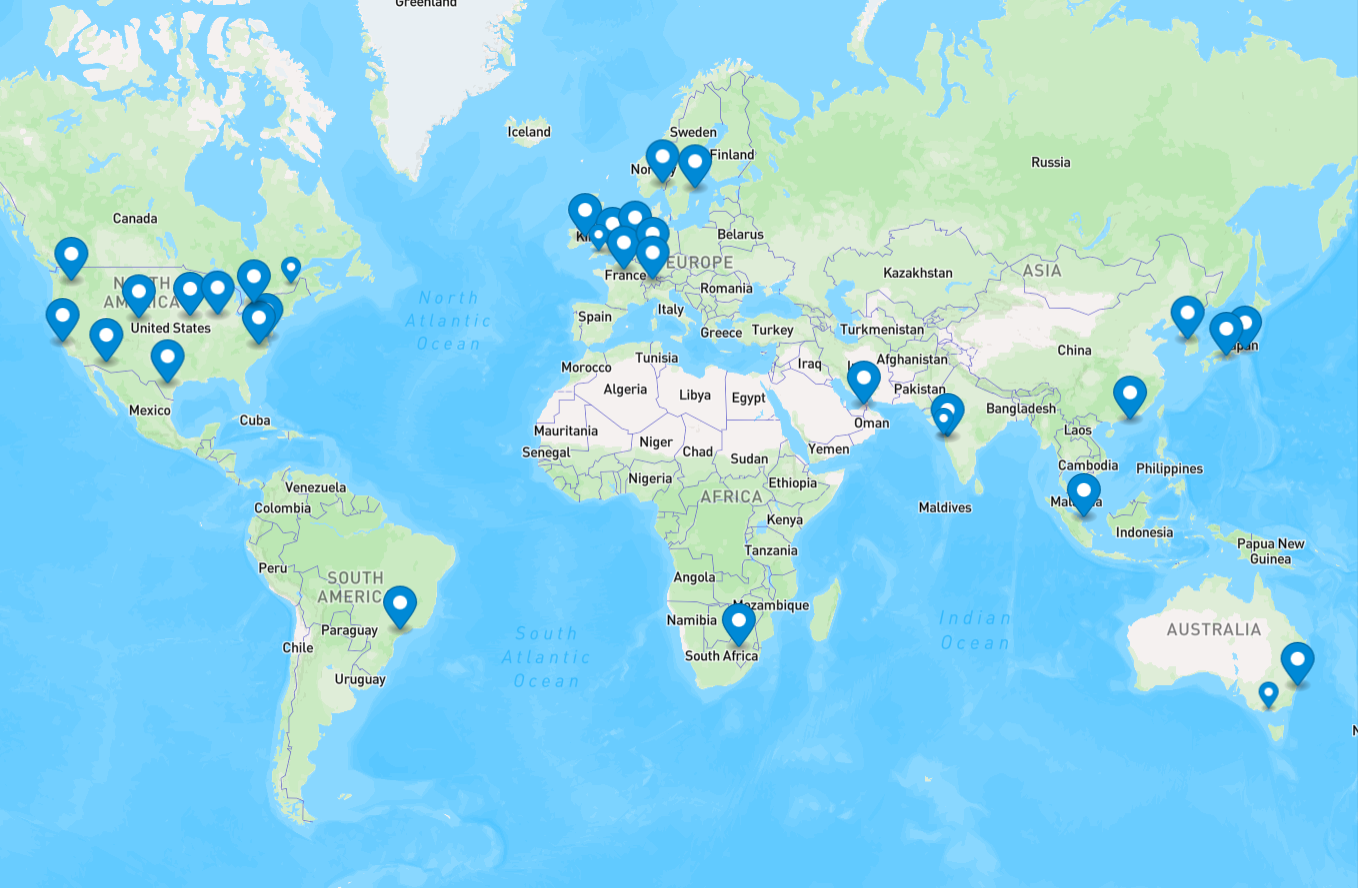
\includegraphics[width=7.5cm]{charts/datacenters_azure.png}}}%
    \qquad
    \subfloat[\centering \GCP]{{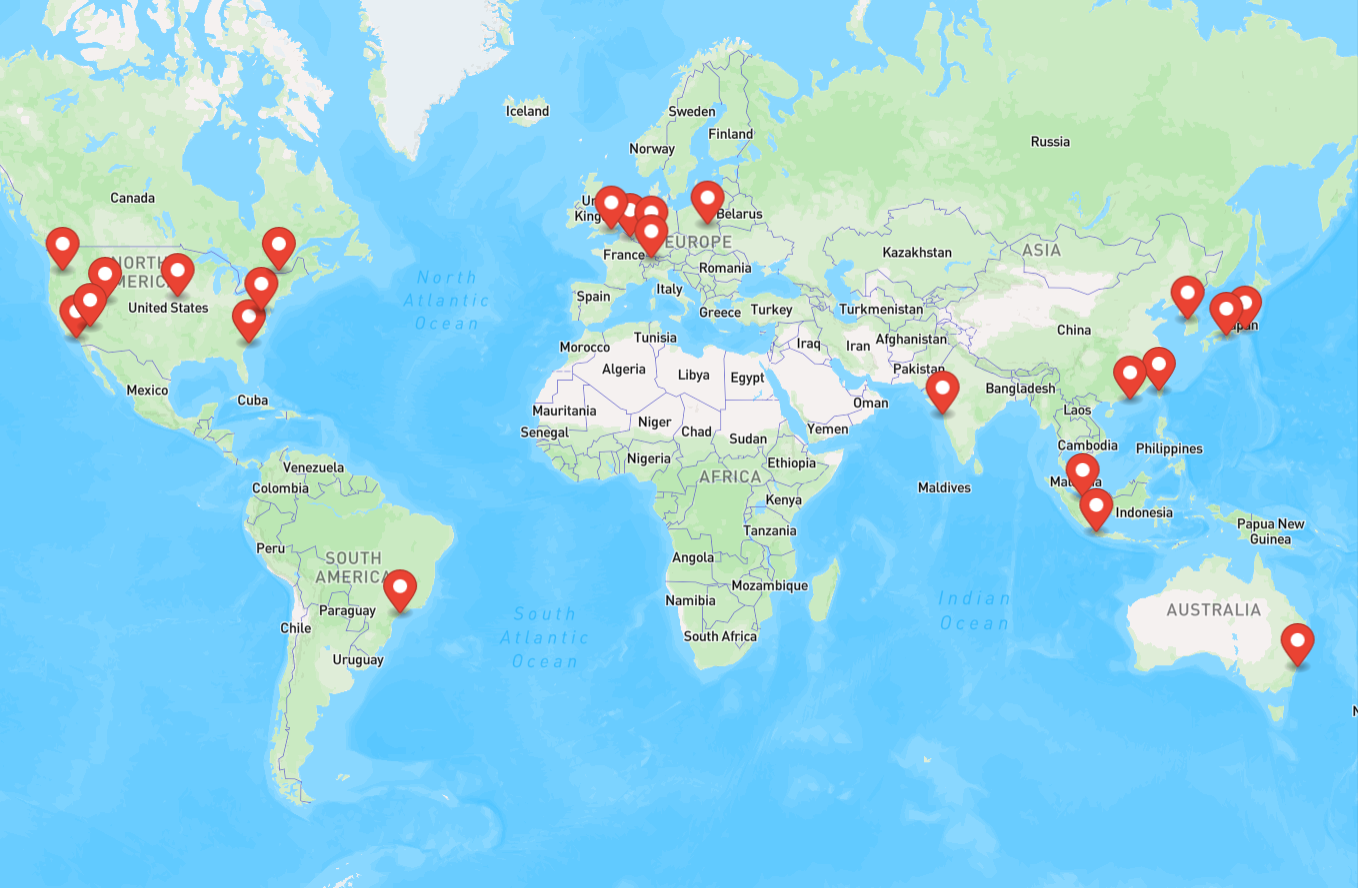
\includegraphics[width=7.5cm]{charts/datacenters_gcp.png}}}%
    \caption{All regions providing FaaS, small pins indicate no OCR support.\\(Map data copyrighted \href{https://www.openstreetmap.org.}{OpenStreetMap} contributors.)}
    \label{fig:regions}
\end{figure}%

\subsection{APIs and SDKs}
In section \ref{sec:files_and_folders} we alluded to an overhead that occurs when using the storage API for file transfer. This also holds for other services, like OCR. Unlike the storage service's API, invoking the OCR service's API cannot be circumvented by publicly available links. As a matter of fact, we cannot even measure transfer times directly at all, rather we regard the service's execution time of the service. For this to work, we need to craft special images (see section \ref{sec:files_images} for more detail) and also call the \textit{REST} API directly.\\
These REST APIs are the 'closest' one can get to the provider, but they require more arguments than needed for performing the service's task itself. In \Azure, OCR for example requires a subscription key,\cite{azure_ocr} \GCP needs an authorization token,\cite{gcp_annotate} and \AWS requires intricate signing altogether.\cite{aws_rekognition} That's why all three providers offer software developer kits (SDKs) for various programming languages, that handle authorization, request signing, target endpoint selection, and so on, before calling the actual REST API.\cite{aws_boto_client,azure_vision_sdk,gcp_annotate_sdk}\\
Behind the scene, these SDKs therefore invoke additional APIs, which add to the total execution time, and especially to latency, rendering SDKs unsuitable for our needs. Moreover, we want to abstract over all programming languages and SDKs, and not compare SDK performance. The solution was to implement the functionality otherwise provided by the SDKs ourselves, but \textit{outside} of the (timed) REST API invocation.

\subsection{Services and OCR}\label{sec:services_ocr}
So far we've always talked about OCR as an example for a service that represents a file transfer endpoint, but it's actually \textit{the} service we picked for measuring performance (alongside each provider's actual file storage service). The reason being that it's the only service where all of the following conditions hold:
\begin{description}
    \item[Available on all three providers.\cite{aws_rekognition,azure_ocr,gcp_annotate}]
    Each provider has its own suite of file related services, from analytics,\cite{aws_analytics} synchronization,\cite{azure_filesync}  migration and even transfer.\cite{gcp_transfer} None of them, however, are comparable across all providers.
    \item[Possibility of restricting the service to a certain region or location.] Some of the aforementioned services operate 'anywhere' in the cloud, or at least outside of the invoker's control. With OCR, the region or location can be restricted using specific endpoints:
    \begin{itemize}
        \item \texttt{rekognition.<region>.amazonaws.com} on \AWS,\cite{aws_ocr_endpoints}
        \item \texttt{<location>.api.cognitive.microsoft.com} on \Azure\cite{azure_ocr_endpoints} and
        \item \texttt{<continent>-vision.googleapis.com} on \GCP.\cite{gcp_ocr_endpoint}
    \end{itemize}
    Admittedly, on \GCP it's a very coarse restriction, but as we've seen in section \ref{sec:endpoints}, \GCP is known for doing routing internally and not offering region-specific endpoints. In fact, when \texttt{vision.googleapis.com} is called from a Google Cloud Function, it resolves to a host within that region, in the same manner as \texttt{storage.googleapis.com} does (see section \ref{sec:endpoints} for details).
    \item[Allowing non-stream input.] Translation services would fulfil all previously mentioned requirements, but their input cannot be a reference to a file. Instead, a string of characters has to be provided,\cite{aws_translate,azure_translate,gcp_translate} which means we would measure transfer speeds between the invoker and the service, not any file transfer. All three OCR services on the other hand, offer either a bucket and object reference,\cite{aws_rekognition} or an arbitrary URL as input.\cite{azure_ocr,gcp_annotate}
    \item[Possibility of crafting suitable input files.] Another time we don't want to measure is the execution time of the service itself, so we don't want OCR to actually be performed. The service therefore has to reject the input file, but only after it has been \textit{fully} read. With a specially crafted image (see section \ref{sec:files_images}), that's possible using the OCR service.
    \item[Synchronous invocation] Speech recognition is another service contender that would comply with our list of requirements so far.\footnote{ID3v2 tags could be used to generate invalid MP3 files with valid prefixed payload.} While \Azure supports synchronous service invocation for short audio files,\cite{azure_speechtotext} \AWS unfortunately only support asynchronous (job-based) invocations.\cite{aws_transcribe} These require multiple API calls and depend on internal scheduling, controlled entirely by the provider, thus not suitable for measuring file transfer times.
\end{description}
Initially, measuring transfer times \textit{across} regions to the OCR service was also considered. But since \AWS doesn't allow this at all (the region of the referenced bucket must match the region of the service)\cite{aws_rekognition_s3} and \GCP only supports continent-level endpoints,\cite{gcp_ocr_endpoint} this plan was scraped, as only \Azure supports fine-grained location restriction and arbitrary input URLs.\cite{azure_ocr,azure_ocr_endpoints}

\subsection{File Operation Capabilities}
To conclude the capabilities sections, we have a look at 'traditional' file operations that providers support. We start with \textit{delete} operations (table \ref{tab:capabilities_delete}).
\begin{table}[ht!]
    \centering
    \begin{tabular}{ |c!{\vrule width 2pt}c|c|c| }
        \hline
        Provider & Retention & \makecell{Restore\\Bucket/Container} & \makecell{Restore\\Object/Blob}\\
        \noalign{\hrule height 2pt}
        \AWS & yes\cite{aws_retention} & \makecell{yes\cite{aws_restore_backup}\\(Amazon Backup)} & \makecell{yes\cite{aws_restore_backup,aws_restore_version}\\(Amazon Backup\\or if versioned)}\\
        \hline
        \Azure & yes\cite{azure_retention} & \makecell{yes\\(from snapshot\cite{azure_restore_container})} & \makecell{yes\cite{azure_restore_blob}\\(from snapshot)}\\
        \hline
        \GCP & yes\cite{gcp_retention} & not documented & \makecell{yes\cite{gcp_restore_version}\\(if versioned)}\\
        \hline
    \end{tabular}
    \caption{Delete operation capabilities.}
    \label{tab:capabilities_delete}
\end{table}%
All providers support retention policies that prevent accidental deletion,\cite{aws_retention,azure_retention,gcp_retention} as well as restoring versioned objects or blobs.\cite{aws_restore_version,azure_restore_blob,gcp_restore_version}
\AWS has a separate backup solution that can also restore buckets,\cite{aws_restore_backup} \Azure uses the same mechanism as it does with blobs.\cite{azure_restore_container}\\
Next we look at \textit{copying} existing cloud objects or blobs (table \ref{tab:capabilities_copy}). Every provider offers APIs to copy objects or blobs across regions,\cite{aws_s3_copyobject,azure_storage_copyblob,gcp_storage_rewrite}. Some of these APIs have a synchronous and asynchronous variant, where some restrictions apply to the former.\cite{aws_s3_copyobject,azure_storage_copyblobfromurl,gcp_storage_copy} In both cases, only entire objects and blobs can be copied, not parts.\cite{aws_s3_copyobject,azure_storage_copyblob,gcp_storage_rewrite}\\
\begin{table}[ht!]
    \centering
    \begin{tabular}{ |c!{\vrule width 2pt}c|c|c| } 
        \hline
        Provider & Across Regions & Synchronous & Partial File\\
        \noalign{\hrule height 2pt}
        \AWS & \makecell{yes\cite{aws_s3_copyobject}\\(with restrictions)} & yes\cite{aws_s3_copyobject} & no\cite{aws_s3_copyobject}\\
        \hline
        \Azure & yes\cite{azure_storage_copyblob} & \makecell{yes\cite{azure_storage_copyblobfromurl}\\(256MB limit)} & no\cite{azure_storage_copyblob,azure_storage_copyblobfromurl}\\
        \hline
        \GCP & yes\cite{gcp_storage_copy} & \makecell{yes\cite{gcp_storage_rewrite,gcp_storage_copy}\\(same region or\\small objects)} & no\cite{gcp_storage_copy,gcp_storage_rewrite}\\
        \hline
    \end{tabular}
    \caption{Copy operation capabilities.}
    \label{tab:capabilities_copy}
\end{table}%
Finally, objects and blobs can be up uploaded in parts or be \textit{constructed} from existing objects. \AWS supports uploading multiple parts of a new object in parallel, and even using (partial) content of existing objects (if those objects are stored in a S3 bucket).\cite{aws_s3_multipart,aws_s3_uploadpartcopy} \Azure goes one step beyond and also supports (partial) external content, where \Azure will download the content from an publicly accessible URL.\cite{azure_storage_putblockfromurl,azure_storage_putpagefromurl}\\
The only provider that cannot use existing content in multipart uploads is \GCP,\cite{gcp_storage_multipartuploads} but - using resumeable uploads - it supports smaller chunks than \AWS at the cost of parallel upload.\cite{gcp_storage_performresumableuploads} \GCP can, however, combine entire existing objects into a new one.\cite{gcp_storage_compose}\\
For a more concise summary see table \ref{tab:capabilities_construct}.
\begin{table}[ht!]
    \centering
    \begin{tabular}{ |c!{\vrule width 2pt}c|c|c|c|c| } 
        \hline
        Provider & Concept & \makecell{From\\Existing\\Objects/\\Blocks} & \makecell{From\\External\\URL} & \makecell{Partial\\Content} & \makecell{Parallel\\Part\\Upload}\\
        \noalign{\hrule height 2pt}
        \AWS & \makecell{Multipart\\Uploads\cite{aws_s3_multipart}} & yes\cite{aws_s3_uploadpartcopy} & no\cite{aws_s3_uploadpart,aws_s3_uploadpartcopy} & \makecell{yes\cite{aws_s3_uploadpartcopy}\\(min. 5MB\\chunks)} & yes\cite{aws_s3_multipart}\\
        \hline
        \Azure & \makecell{Block or\\Page Blob\cite{azure_storage_blobs}} & yes\cite{azure_storage_putblockfromurl,azure_storage_putpagefromurl} & yes\cite{azure_storage_putblockfromurl,azure_storage_putpagefromurl} & \makecell{yes\\(blocks\cite{azure_storage_putblockfromurl} or\\pages\cite{azure_storage_putpagefromurl})} & yes\cite{azure_storage_putblocklist}\\
        \hline
        \multirow{3}{*}[-2.5em]{\GCP} & \makecell{Multipart\\Uploads\cite{gcp_storage_multipartuploads}} & no\cite{gcp_storage_uploadpart} & no\cite{gcp_storage_uploadpart} & \makecell{yes\\(min. 5MB\\chunks\cite{gcp_storage_quotas})} & yes\cite{gcp_storage_multipartuploads}\\
        \cline{2-6}
        & \makecell{Resumable\\Uploads\cite{gcp_storage_resumableuploads}} & no\cite{gcp_storage_performresumableuploads} & no\cite{gcp_storage_performresumableuploads} & \makecell{yes\\(multiple\\of 256KB\cite{gcp_storage_performresumableuploads})} & no\cite{gcp_storage_performresumableuploads}\\
        \cline{2-6}
        & \makecell{Combine\\Objects\cite{gcp_storage_compose}} & yes\cite{gcp_storage_compose} & no\cite{gcp_storage_compose} & no\cite{gcp_storage_compose} & \makecell{yes\cite{gcp_storage_compose}\\(objects\\as parts)}\\
        \hline
    \end{tabular}
    \caption{Construct (from parts) operation capabilities.}
    \label{tab:capabilities_construct}
\end{table}%

\section{Test Environment}\label{sec:testenv}
Equipped with the knowledge about transfer capabilities and the challenges of measuring transfer times, we now explore the practical solutions to these problems in our \textit{Cloud Workbench}.\cite{wb} We will also provide information on how to setup the environment, and how to extend it.

\subsection{Design Goals}
In general, the design goals behind the test environment where flexibility, extendibility and economics. Let's start with the last one, as it explains the architecture from the bottom up.

\subsubsection{Economics}
Since we want to measure transfer times across the globe and between all three providers, we need to able to execute code in every region of every provider. Traditionally, this would require almost 100 virtual machines,\cite{aws_regions,azure_regions,gcp_regions} which entails the time and cost of deploying, running and managing VMs, as well as implementing some sort of job dispatching. That's why we opted for a serverless solution using functions as a service (FaaS).\cite{faas_introduction} Not only does it allow us to directly invoke test code, each provider also offers millions of free invocation each month.\cite{aws_lambda,azure_functions,gcp_functions}

\subsubsection{Flexibility}
While using FaaS takes care of the costs and managing VMs, deploying the functions is still a time consuming process. Redeploying functions is usually a bit faster, but the initial deployment can take several minutes.\cite{gcp_function_deployment} This doesn't allow for much flexibility as far as code changes are concerned, especially when you have to deploy to hundreds of regions on different providers.\\
Our solution to this problem is using a single JavaScript (NodeJS) function, that is able to dynamically execute submitted code.\cite{wb_aws_function,wb_azure_function,wb_gcp_function} Not only is redeployment time reduced to zero, it also allows for shared code between providers. As figure \ref{fig:function} shows, most of the function itself is common across all three providers as well.
\begin{figure}[!ht]
\begin{lstlisting}[style=ES6]
try {
  if (typeof request !== 'object')
    return badRequest('Body must be a JSON object.')
  if (typeof request.time !== 'number')
    return badRequest('Time must be a number.')
  if (Math.abs(Date.now() - request.time) > 60000)
    return badRequest('Time difference is too big.')
  if (typeof request.command !== 'string')
    return badRequest('Command must be a string.')
  if (typeof request.hash !== 'string')
    return badRequest('Hash must be a string.')
  if (typeof key !== 'string' || key.length < 16)
    return internalServerError('Invalid key.')
  const { createHmac } = await import('node:crypto')
  const hmac = createHmac('sha256', key)
  hmac.update(`<${request.time}|${request.command}>`)
  if (hmac.digest('hex') !== request.hash)
    return forbidden('Hash mismatch.')
  return success(await AsyncFunction(request.command).call(null))
} catch (e) {
  return internalServerError(String(e))
}
\end{lstlisting}
\caption{Common code of FaaS functions.}
\label{fig:function}
\end{figure}%
What differs is how errors are signalled to the executing runtime (\texttt{badRequest}, \texttt{forbidden}, etc.) and the way the result is returned upon \texttt{success}.\\
To ensure that commands cannot be executed by anyone, rather than relying on a simple app key that gets appended to each query,\cite{azure_functions_keys} we employ HMAC using a secret key, that never gets transmitted. Both command and current time get hashed, so even if a request would somehow get intercepted, it can only be repeated in a very short time frame. An adversary can, however, never alter the command without invaliding the HMAC.\cite{hmac}

\subsubsection{Extendibility}
The last goal was to ensure that the test environment can be extended without having to deal with any of the aforementioned internals. Also, it should be easy to use it in a scripting language, both of which is achieved by a PowerShell file that can be \textit{dot-included} by running \texttt{. ./invoke.ps1}.\cite{wb_invoke} After doing so, getting for example the NodeJS version for all regions in all providers is as simple as invoking
\begin{verbatim}
$All | Invoke-CloudFunction -Command "return process.version" -Raw
\end{verbatim}
where \texttt{\$All} and \texttt{Invoke-CloudFunction} are provided by the script. Instead of \texttt{\$All} for all providers, \texttt{\$Azure}, \texttt{\$AWS} and \texttt{\$GCP} can be used as well. Or, to speed things up, execute \texttt{Invoke-CloudFunction} in parallel:
\begin{verbatim}
$All | % -ThrottleLimit 20 -Parallel {
  . ./invoke.ps1
  $_ | Invoke-CloudFunction -Command "return process.version" -Raw
}
\end{verbatim}
Since the command is just JavaScript, it can be dynamically generated by using string variables. The script for example exports \texttt{\$GCP\_StorageBucket}, which creates a \GCP storage object and selects the bucket in the region of the function. Checking if an object named \textit{waldo.txt} exists in region \textit{us-west1} can therefore be written as:
\begin{verbatim}
Invoke-CloudFunction -Provider GCP -Region us-west1 -Command `
  "return await $GCP_StorageBucket.file('waldo.txt').exists()"
\end{verbatim}
So extending the test environment is as easy as defining and using string variables.

\subsection{Deployment}
To get the test environment up and running, we provide three \texttt{prepare.sh} scripts:
\begin{description}
    \item[\AWS\cite{wb_aws_prepare}] This script asks the user for a prefix and creates Lambda functions\cite{aws_lambda} and S3 buckets in configured\cite{wb_aws_regions} \AWS regions, using the provided prefix and the region to generate the bucket name.
    \item[\Azure\cite{wb_azure_prepare}] Executing the script queries for the name of an \Azure resource group,\cite{azure_resouce_groups} its primary location and the container name to be used. It then creates the resource group, as well as storage accounts, containers and function apps\cite{azure_functions} for all configured\cite{wb_azure_regions} locations. The length of the resource group's name added to the length of the longest location name must not exceed 24 characters, as this is the maximum storage account name length,\cite{azure_storage_account} and also how the name of storage accounts are generated. 
    \item[\GCP\cite{wb_gcp_prepare}] As with the two previous scripts, functions\cite{gcp_functions} and buckets are created for configured\cite{wb_gcp_regions} regions. As prefix the name of the \GCP project\cite{gcp_projects} is queried and used.
\end{description}
All three scripts will install the provider's CLI if it's not present. In addition, they create the necessary permissions, roles and policies for accessing the buckets/containers publicly and being able to write to them using the provider's FaaS solution.\\
In addition there are also three \texttt{update.sh} scripts, which will redeploy all functions and settings if needed.\cite{wb_aws_update,wb_azure_update,wb_gcp_update}

\subsection{Files and Images}\label{sec:files_images}
After deployment, the buckets and containers are filled using the \texttt{Initialize-CloudFiles} function exported by the invocation script.\cite{wb_invoke} Figure \ref{fig:files} shows the lines that define what files are being created.
\begin{figure}[!ht]
\begin{lstlisting}[style=ES6]
const sizes = [512, 10*1024, 1024*1024, 10*1024*1024]
const files = [
  ['zero.bin', () => Buffer.alloc(0)],
  ['image_ping.png', () => png(() => null, 0)],
  ['image_full.png', () => png(() => randomBytes(10*1024), 408)],
  ...sizes.flatMap(size => [
    [`zero_${size}.bin`, () => Buffer.alloc(size)],
    [`random_${size}.bin`, () => randomBytes(size)]
  ])
]
\end{lstlisting}
\caption{File specifications in \texttt{Initialize-CloudFiles}.\cite{wb_invoke}}
\label{fig:files}
\end{figure}%
As you can see, the files being generated are 512B, 10KiB, 100KiB and 10MiB in size, one set with random bytes, one with all zeros, as well as one empty file and two images.\\
The images are created using the \texttt{png} function, which takes as argument a function \texttt{chunkData} a number \texttt{count}, and returns an invalid PNG image. A PNG image is made of chunks of variable size, and supports public as well as private chunks, "to carry data that is not of interest to other applications".\cite{png} Precisely such a chunk, named \textit{fiLl}, is created using data returned from the \texttt{chunkData} function, and placed in the image \texttt{count} times. The capitalization in \textit{fiLl} indicates that these chunks are ancillary, private and safe to copy,\cite{png} so a parser will read and ignore them.\\
Valid PNG files start with a specific signature, followed by an \textit{IHDR} chunk describing the image, contain at least one \textit{IDAT} chunk carrying the image data, and end with a \textit{IEND} chunk.\cite{png} The files returned by \texttt{png} also start with the signature and an \textit{IHDR} chunk (indicating a 1000x1000 pixel RGB image), followed by \texttt{count} \textit{fiLl} chunks and the final \textit{IEND} chunk. There is, however, no \textit{IDAT} chunk, which the cloud provider's image parser only knows after reading all the \textit{fiLl} chunks, when it encounters \textit{IEND}. The reason why multiple \textit{fiFl} chunks are used is to ensure that the parser cannot just seek over one big \textit{fiLl} chunk. Ideally, the size of one \textit{fiLl} chunk matches the parser's read buffer size.\\
\\
Once all tests are run (and to prevent unnecessary storage cover charges), \texttt{Clear-CloudFiles} can be used to delete all files from buckets/containers. \texttt{Copy-CloudFile} provides the ability to upload data from a local machine or download a file from some other location into a bucket or container, and \texttt{Test-CloudFile} checks if a file exists. All commands take as argument the name of a provider and region, and - just like \texttt{Invoke-CloudFunction} - can be piped in one of the helper variables \texttt{\$All}, \texttt{\$AWS}, \texttt{\$Azure} or \texttt{\$GCP}.

\section{Results}
The following results were generated using the test environment described in section \ref{sec:testenv}. The file tests ran across 22 \AWS regions,\cite{wb_aws_regions}, 32 \Azure locations,\cite{wb_azure_regions} and 23 \GCP regions,\cite{wb_gcp_regions} depicted in figure \ref{fig:regions}. OCR tests were performed on all \GCP regions and a subset of \AWS (12\cite{wb_aws_regions_ocr}) and \Azure(28\cite{wb_azure_regions_ocr}).

\subsection{File Transfer}\label{sec:fileresults}
As described in section \ref{sec:files_images} and shown in figure \ref{fig:files}, 9 different files with 5 different sizes where used in the test. \texttt{Test-CloudFileTransfer}\cite{wb_invoke} was invoked with all possible combinations of regions, and at three different times: 12:00 Central European Time, 12:00 Japan Standard Time and 12:00 Eastern Standard Time. All $9*(22+32+23)^2*3=160083$ data points are publicly available.\cite{wb_results_file}\\
\begin{figure}[!ht]
    \centering
    \includesvg[pretex=\scriptsize,width=0.75\textwidth]{charts/main.svg}
    \caption{Average transfer time between providers.}
    \label{fig:main}
\end{figure}%
Figure \ref{fig:main} shows the average transfer times over all different files, times and regions between providers. While downloading from \Azure takes more or less the same time across all providers, transfer speeds between \AWS and \GCP are definitely not symmetrical. Interestingly, transferring from \GCP to itself takes almost double the time than to \Azure. Let's see if any of the components we averaged over can provide further explanation.\\
First we look at the same results but split up into the three different times of day in figure \ref{fig:noon}.
\begin{figure}[!ht]
    \centering
    \subfloat[\centering 12:00 CET]{{\includesvg[pretex=\fontsize{3}{3.6}\selectfont,width=5.25cm]{charts/noon_eu.svg}}}%
    \enspace
    \subfloat[\centering 12:00 JST]{{\includesvg[pretex=\fontsize{3}{3.6}\selectfont,width=5.25cm]{charts/noon_jp.svg}}}%
    \enspace
    \subfloat[\centering 12:00 EST]{{\includesvg[pretex=\fontsize{3}{3.6}\selectfont,width=5.25cm]{charts/noon_us.svg}}}%
    \caption{Average transfer time between providers at different times.}
    \label{fig:noon}
\end{figure}%
Alas, but also unsurprisingly, these plots add no further insight, as the average transfer times remain almost the same. They are, after all, still averaged over all regions.\\
Next let's look at the different file types in figure \ref{fig:type}.
\begin{figure}[!ht]
    \centering
    \subfloat[\centering Empty 'ping' files.]{{\includesvg[pretex=\fontsize{3}{3.6}\selectfont,width=5.25cm]{charts/type_ping.svg}}}%
    \enspace
    \subfloat[\centering Files containing all zeroes.]{{\includesvg[pretex=\fontsize{3}{3.6}\selectfont,width=5.25cm]{charts/type_zero.svg}}}%
    \enspace
    \subfloat[\centering Files containing random bytes.]{{\includesvg[pretex=\fontsize{3}{3.6}\selectfont,width=5.25cm]{charts/type_random.svg}}}%
    \caption{Average transfer time between providers using different file types.}
    \label{fig:type}
\end{figure}%
Here we can see the first significant difference to figure \ref{fig:main}: Empty files, which can be seen as the equivalent to doing a \textit{ping} at the storage level, take (almost) the same to every provider. Although 'pinging' \AWS storage takes longer than \GCP's, there is no outlier like in figure \ref{fig:main}. Yet the same outlier appears again for non-empty files. The difference between files containing random bytes and all zeroes seems to make no difference, except when downloading from \GCP. Let's explore these two observations further.\\
\begin{figure}[!ht]
    \centering
    \includesvg[pretex=\scriptsize,width=0.75\textwidth]{charts/sizes.svg}
    \caption{Average transfer time between providers by file size.}
    \label{fig:sized}
\end{figure}%
Figure \ref{fig:sized} combines the file types again, but shows the average transfer time by each file size. At first glance it may appear as if transfers from \AWS to \GCP actually scale exponentially in size, but at closer inspection, it becomes apparent that all other transfers just pick up speed faster (c.f. TCP slow start\cite{tcp_congestion}). While blackbox testing cannot fully uncover the reason behind it, it is likely that some artificial rate limiting is employed, as downloading from \Azure to \GCP doesn't show this behavior.\\
The difference between files of 0, 512 and 10240 bytes in size across all three providers is negligible, which makes sense since these amounts can be transferred in one packet\footnote{With possible fragmentation, except for jumbograms.\cite{jumbograms}}, hence all act more or less as 'ping'. But let's have a closer look at the difference between files containing random data and all zeroes again.\\
\begin{figure}[!ht]
    \centering
    \subfloat[\centering Files containing all zeroes.]{{\includesvg[inkscapelatex=false,width=17cm]{charts/area_zero.svg}}}%
    \qquad
    \subfloat[\centering Files containing random bytes.]{{\includesvg[inkscapelatex=false,width=17cm]{charts/area_random.svg}}}%
    \caption{Average transfer time between providers and regions.}
    \label{fig:area}
\end{figure}%
To illustrate the difference, figure \ref{fig:area} shows a 3d surface of average transfer times between all regions,\footnote{Except for \textit{southafricanorth} and \textit{australiaeast} on \Azure to improve visibility.} once for each file type (except empty files). While transfers from other providers seem unaffected, downloading files containing all zeroes - i.e. compressible files - from \GCP results in shorter download times. If we consider section \ref{sec:endpoints} and the fact that \GCP transfers files internally over most of the path between the data center and the client, it is likely to assume some compression is indeed employed by the provider.\\
This concludes the file result section. Of course there are facets to explore (see section \ref{sec:future}), let's move on to the OCR results nonetheless.

\FloatBarrier
\subsection{OCR Transfer}\label{ocrresults}
As mentioned in section \ref{sec:services_ocr}, measuring OCR transfer was done using the recognition service and storage of the same regions. \texttt{Test-CloudOcrTransfer}\cite{wb_invoke} was invoked with all 63 OCR-supporting regions twice, once at 00:00 UTC, and again at 12:00 UTC. Each invocations tests the file transfer and OCR execution speed of \textit{image\_ping.png} and \textit{image\_full.png} (see section \ref{sec:files_images}) five times in a row, which we will call the five \textit{requests} from here on out. All $63*2*2*2*5=2520$ data points are publicly available.\cite{wb_results_ocr} Figure \ref{fig:ocr_main} aggregates over regions, time and requests.\\
\begin{figure}[!ht]
    \centering
    \includesvg[pretex=\tiny,width=0.66\textwidth]{charts/ocr_main.svg}
    \caption{Average download time (OCR=FALSE) vs OCR execution time (OCR=TRUE).}
    \label{fig:ocr_main}
\end{figure}%
The values for OCR on \textit{image\_ping.png} show an expected higher overhead of invoking the service, while the non-OCR values correspond to the previous file tests. Looking at \textit{image\_full.png}, the first observation is that every provider offers faster transfers between the OCR service and the storage than between FaaS and the storage within each region. While not immediately obvious from figure \ref{fig:ocr_main}, this also holds true for \Azure, as we have to subtract the OCR overhead and thus end up with a lower invocation time.\\
The second observation is that the download times returned by \texttt{Test-CloudOcrTransfer} are slightly higher than those of \texttt{Test-CloudFileTransfer} (c.f. section \ref{sec:fileresults}). This can be attributed to the fact that the former uses \textit{fetch} and parses the results, while the latter uses the \textit{node:https} module and discards downloaded chunks.\cite{wb_invoke} There is also a slight delay during the first request, as can be seen in figure \ref{fig:batch} for \textit{image\_ping.png}. However, when fetching or running OCR on the full image, the delay becomes negligible.\\
\begin{figure}[!ht]
    \centering
    \subfloat[\centering \textit{image\_ping.png}]{{\includesvg[pretex=\fontsize{4}{4.8}\selectfont,width=7.5cm]{charts/ocr_batch_ping.svg}}}%
    \qquad
    \subfloat[\centering \textit{image\_full.png}]{{\includesvg[pretex=\fontsize{4}{4.8}\selectfont,width=7.5cm]{charts/ocr_batch_full}}}%
    \caption{Average transfer time for each request.}
    \label{fig:batch}
\end{figure}%
While more comparisons - e.g. time of day or performance per region - could be shown, the results are similar to those presented in the previous section and therefore omitted for brevity.

\section{Corollary and Future Work}\label{sec:future}
The findings presented in section \ref{sec:fileresults} are only a fraction of what can be gathered from the collected data. While we have shown that transfer speed between providers cannot be assumed to be symmetric, we only focused on the provider level. Yet, as figure \ref{fig:intraprovider} shows, there is clearly more to uncover at a regional level, since transferring between \GCP regions is definitely not symmetrical either, unlike on \AWS and \Azure.\\
In multi-provider deployments, our OCR service results (section \ref{ocrresults}) can help decide which provider and region to target, depending on the image size. The next step here would be to run the tests across providers as well. While this won't work with \AWS, \Azure and \GCP can download source images from anywhere, as we've discussed in section \ref{sec:services_ocr}. Based on those results, schedulers could decide to either first transfer the file via storage and invoke the service within the same region, or let the service download it directly.\\
Another topic of interest not covered so far is the relation between geolocation and file transfers. While measuring transfer time and bandwidth has been used to calculate the location of a host before,\cite{geolocation1,geolocation2} it would be interesting to see if enriching those methods with our approximately 6000 known triples of latency, bandwidth and distance can help improve accuracy.\\
Regarding bandwidth, we've seen that there is a stark difference in how transfers increase throughput with larger file size in section \ref{sec:fileresults}. However, since the largest files were only 10MiB in size, it is very likely that our tests did not uncovered the maximum bandwidth. The reason for not using larger files was simple economics, as transfers aren't cheap,\cite{azure_bandwidth_costs} and, due to our full-mesh tests, scale exponentially in size. Running the tests again with a higher budget and simply changing one line (see section \ref{sec:files_images}) would fill the gap.\\
Finally, all transfers in our tests so far have been downloads. And while figure \ref{fig:intraprovider} suggests that those are symmetrical within \Azure locations, initial tests have shown that this is not true for \textit{uploading} data. That is to say that the speed with which region A downloads from region B, is not the same as region B uploads to region A. Especially in multi-regional deployments, knowing about these asymmetries can help schedulers decide \textbf{how} to move data, which until now just focused on \textbf{where} to move it to.\\
\\
In any case, our Cloud Workbench can be used to implement and run future tests.

\begin{figure}[!ht]
    \centering
    \subfloat[\centering \AWS]{{\includesvg[inkscapelatex=false,width=5cm]{charts/region_aws.svg}}}%
    \quad
    \subfloat[\centering \Azure]{{\includesvg[inkscapelatex=false,width=5cm]{charts/region_azure.svg}}}%
    \quad
    \subfloat[\centering \GCP]{{\includesvg[inkscapelatex=false,width=5cm]{charts/region_gcp.svg}}}%
    \caption{Average transfer time between regions.}
    \label{fig:intraprovider}
\end{figure}%

\newpage
\bibliographystyle{unsrtnat}
\bibliography{refs}

\end{document}
